\documentclass{article}
\usepackage{fullpage,amssymb,amsmath,amsthm,url,graphicx}

\begin{document}


\section*{Local parameterizations}

Let $L_\tau(\tau):=E_{q(w|\tau)}[\ell(w)]$.
Ordinary NGD with respect to global parameter $\tau$ is
$$
\tau_{t+1} = \tau_t-\beta F_\tau^{-1}(\tau_t) \nabla_\tau L_\tau(\tau_t),
$$
where $\beta$ is the learning rate.
Using local parameterization $\eta$ and auxiliary parameterization $\lambda_t$ 
with $\tau_\eta=\psi\circ\phi_{\lambda_t}$ so that $\tau_\eta(\eta)=\tau$ at iteration $t$ via $\lambda_t$, 
we have one iteration of NGD with respect to local parameterization $\eta$ as:
$$
\eta'=\eta_0-\beta F_\eta^{-1}(\eta_0) \nabla_\eta L_\eta(\eta_0)
$$
Since we choose $\eta_0=0$, and we have $L_\eta=L_\tau \circ \tau_\eta$, we get using the chain rule (a multivariate generalization of  $f(g(y))'=g'(y)f'(g(y))$ with $x=g(y)$):
\begin{eqnarray*}
\eta' &=& -\beta F_\eta^{-1}(\eta_0)   \left(\nabla_\eta (L_\tau \circ \tau_\eta)(\eta_0)\right) \\
&=& -\beta F_\eta^{-1}(\eta_0)  \left(\nabla_\eta (\psi\circ\phi_{\lambda_t})(\eta_0)\right) \nabla_\tau L_\tau(\tau)
\end{eqnarray*}
Then we map back $\eta'$ to $\tau$ as 
$$
\tau_{t+1}=\tau_\eta(\eta')=\psi\circ\phi_{\lambda_t}\left(
-\beta F_\eta^{-1}(\eta_0)  (\nabla_\eta (\psi\circ\phi_{\lambda_t})(\eta_0)) \nabla_\tau L_\tau(\tau)
\right)
$$

\begin{figure}
\centering
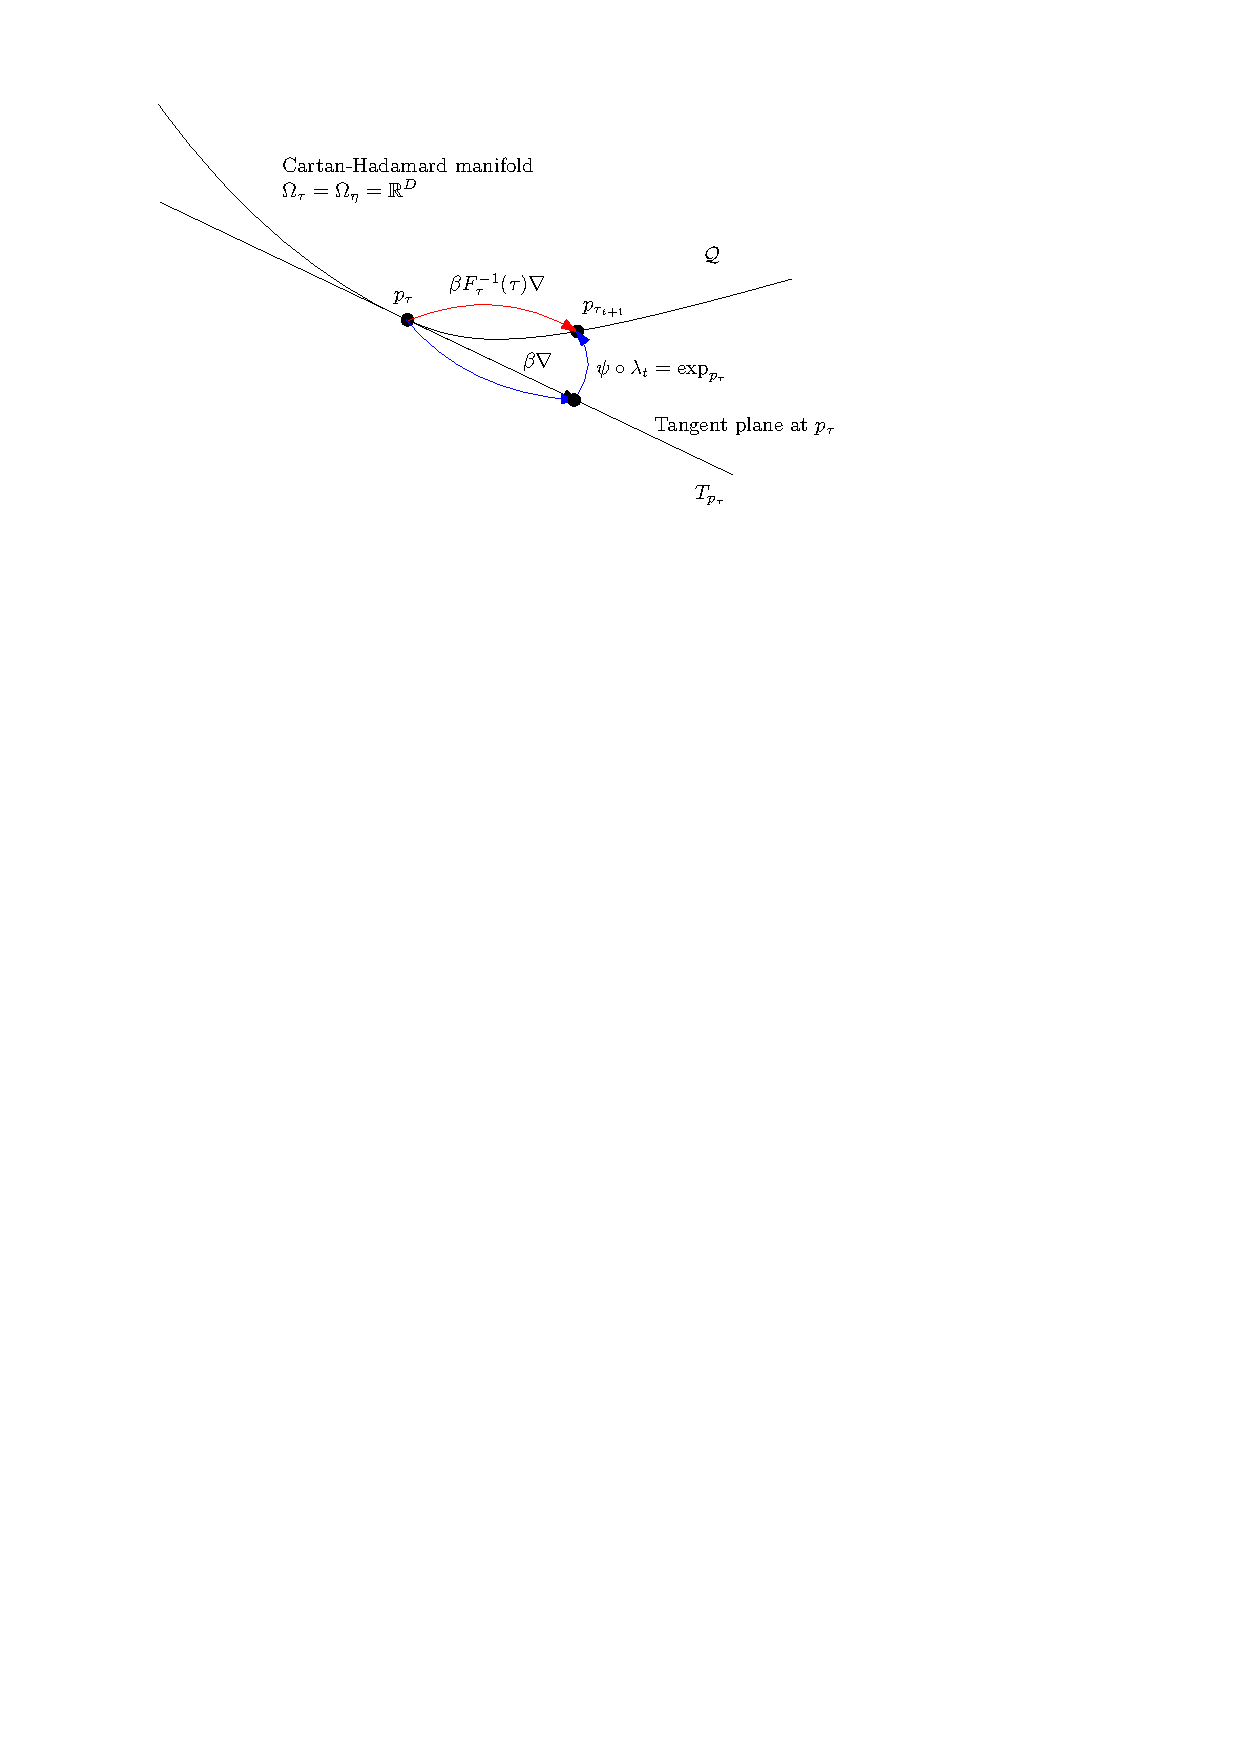
\includegraphics[width=0.7\textwidth]{FigIpe-LocalNaturalCoordinatesCartanHadamardMfd.pdf}
\caption{Geometric interpretation of local natural coordinates on a Cartan-Hadamard manifold.}\label{fig:geointerpretation}
\end{figure}

%%
\subsection{The case of Cartan-Hadamard manifolds}
%%%
When the Fisher-Rao $D$-dimensional manifold $\mathcal{Q}$ is a Cartan-Hadamard manifold (non-positive sectional curvature like the manifold of positive-definite matrices)
then by Cartan?Hadamard theorem the manifold is diffeomorphic to $\mathbb{R}^D$.
In a Cartan-Hadamard manifold, the Riemannian exponential map $\exp_p:T_p\mathcal{Q}\rightarrow\mathcal{Q}$ is a covering map.
Thus we can choose $\eta$ to be the Euclidean coordinates in the tangent plane $T_p$ with ordinary gradient, and define $\psi\circ\lambda_t(\eta)=\exp_{p_{\tau_t}}(v)$ to be the Riemannian exponential map. 
Therefore on any  Fisher-Rao manifold which is of Cartan type (e.g., manifold of Gaussians), we can introduce local natural coordinates.
Notice that when the FIM is constant, $F_\eta^{-1}(\eta_0)$, then by a change of variable using Cholesky decomposition, we can make it 
 Euclidean. Figure~\ref{fig:geointerpretation} gives a geometric intepretation of the local natural coordinates on such manifolds.

\end{document}

 